%\section{Background and related work}
\label{ch3:background}

In this chapter, we discuss the related work with respect to FAIR Digital Objects and Linked Data. We do so by looking through the lens of development of these technologies over time, including future directions.

\section{FAIR Digital Object}\label{ch3:fdo}


In brief, the structure of a FAIR Digital Object (FDO) is to, given a \emph{persistent identifier} (PID) such as a DOI, resolve to a \emph{PID Record} that gives the object a \emph{type} along with a mechanism to retrieve its \emph{bit sequences}, \emph{metadata} and references to further programmatic \emph{operations} (figure \vref{ch3:fig:fdo}). The type of an FDO (itself an FDO) defines attributes to semantically describe and relate such FDOs to other concepts (typically other FDOs referenced by PIDs). The premise of systematically building an ecosystem of such digital objects is to give researchers a way to organise complex digital entities, associated with identifiers, metadata, and supporting automated processing \cite{wittenburgDigitalObjectsDrivers2019a}.


%%

The concept of \textbf{FAIR Digital Objects} \cite{Schultes 2019} has been introduced as a way to expose research data as active objects that conform to the FAIR principles \cite{Wilkinson 2016}. This builds on the \emph{Digital Object} (DO) concept \cite{Kahn 2006}, first introduced by \cite{kahnFrameworkDistributedDigital1995a} as a system of \emph{repositories} containing \emph{digital objects} identified by \emph{handles} and described by \emph{metadata} which may have references to other handles. DO was the inspiration for the \cite{x1255FrameworkDiscovery} framework which introduced an abstract \emph{Digital Entity Interface Protocol} for managing such objects programmatically, first realised by the Digital Object Interface Protocol (DOIP) \cite{DigitalObjectInterface}.

In brief, the structure of a FAIR Digital Object (FDO) is to, given a \emph{persistent identifier} (PID) such as a DOI, resolve to a \emph{PID Record} that gives the object a \emph{type} along with a mechanism to retrieve its \emph{bit sequences}, \emph{metadata} and references to further programmatic \emph{operations} (figure \vref{ch3:fig:fdo}). The type of an FDO (itself an FDO) defines attributes to semantically describe and relate such FDOs to other concepts (typically other FDOs referenced by PIDs). The premise of systematically building an ecosystem of such digital objects is to give researchers a way to organise complex digital entities, associated with identifiers, metadata, and supporting automated processing \cite{wittenburgDigitalObjectsDrivers2019a}.
As mentioned previously, this ecoystem is envisioned to consist of a wide variety of digital entities and contextual information ranging from software to articles to even descriptions of experimental infrastructures \cite{Azeroual2022PuttingFP}.
Recently, it has been noted that the practical use of FDOs to achieve interoperability requires governance in particular with respect to assessing such interoperability \cite{Wilkinson2023}.

FDOs have been recognised by the European Open Science Cloud (\href{https://eosc.eu/}{EOSC}) as a suggested part of its Interoperability Framework \cite{eosc-interop-framework}, in particular for deploying active and interoperable FAIR resources that are \emph{machine actionable}. Development of the FDO concept continued within Research Data Alliance (\href{https://www.rd-alliance.org/}{RDA}) groups and EOSC projects like \href{https://www.go-fair.org/}{GO-FAIR}, concluding with a set of guidelines for implementing FDO \cite{bonino2019}. The \href{https://fairdo.org/}{FAIR Digital Objects Forum} has since taken over the maturing of FDO through focused working groups which have currently drafted several more detailed specification documents \cite{fdo-Specs}.
%%


\begin{figure}[hbt]
  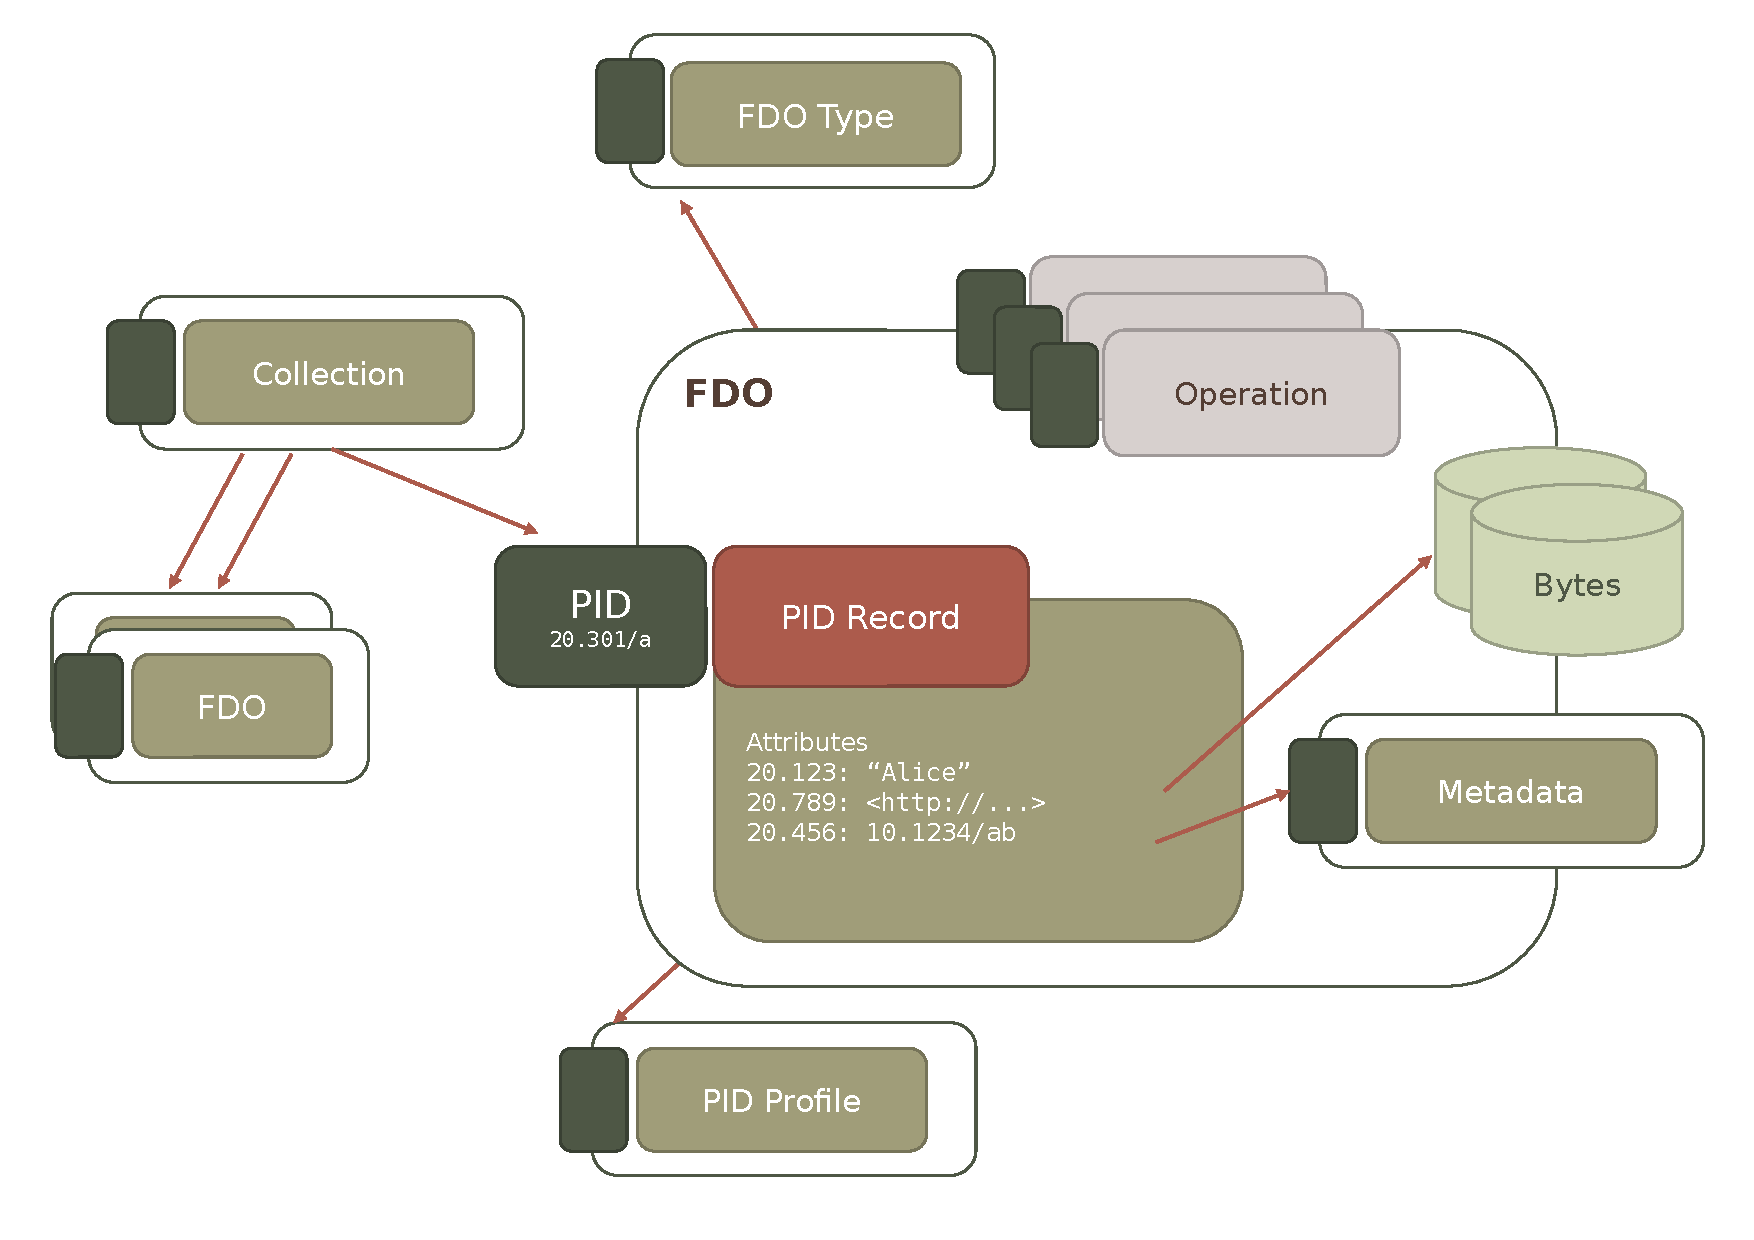
\includegraphics[width=\textwidth]{figures/ch03/fdo.pdf}
    \caption[Idealised overview of a FAIR Digital Object]{\textbf{Idealised overview of a FAIR Digital Object}. The persistent identifier (PID), (e.g. a Handle, DOI or permalink), refers to an FDO through a PID Record, which may reference downloadble bytes, and optionally additional metadata in another FDO. A series of operations are accessible from an FDO (for instance retrieving the bytes). Similar to in object-oriented programming, the FDO Type indicates which operations and attributes are applicable to an FDO. FDOs can be cross-related using the PIDs, a Collection is then another such FDO which aggregates other FDOs by reference. The configuration shown here is just one of many possible \cite{fdo-ConfigurationTypes}, along with the choice of PID system, nature of the PID Record and metadata vocabularies, which are identified through an FDO Profile. In practice, some compromises from this idealised picture are taken depending on the implementation, for instance attribute keys may be simple strings rather than PIDs, and default operations are not explicitly declared.
    }
  \label{ch3:fig:fdo}
\end{figure}

Recently, FDOs have been recognised by the European Open Science Cloud \footurl{https://eosc.eu/}{(EOSC)} as a suggested part of its Interoperability Framework \cite{eosc-interop-framework}, in particular for deploying active and interoperable FAIR resources that are \emph{machine actionable}. Development of the FDO concept continued within Research Data Alliance \footurl{https://www.rd-alliance.org/}{(RDA)} groups and EOSC projects like \footurl{https://www.go-fair.org/}{GO-FAIR}, concluding with a set of guidelines for implementing FDO \cite{bonino2019}. The \footurl{https://fairdo.org/}{FAIR Digital Objects Forum} has since taken over the maturing of FDO through focused working groups which have currently drafted several more detailed specification documents (see \emph{Next steps for FDO} \vpageref{ch3:next-step-fdo}).

\subsection{FDO approaches}\label{ch3:fdo-approaches}

FDO is an evolving concept. A set of FDO Demonstrators \cite{wittenburgFAIRDigitalObject2022b} highlights how current adapters are approaching implementations of FDO from different angles:

\begin{itemize}
\tightlist
\item
  Building on the Digital Object concept, using the simplified DOIP v2.0 \cite{DONA 2018} specification, which detail how to exchange JSON objects through a text-based protocol\footnote{For a brief introduction to DOIP 2.0, see \cite{DOIPExamplesCordraa}} (usually TCP/IP over TLS). The main DOIP operations are retrieving, creating and updating digital objects. These are mostly realised using the reference implementation Cordra \cite{tupelo-schneckrobertBriefIntroductionCordra2022}. FDO types are registered in the local Cordra instance, where they are specified using JSON Schema \cite{Draftbhuttonjsonschema} and PIDs are assigned using the Handle system. Several type registries have been established.
\item
  Following the Linked Data approach, but using the DOIP protocol, e.g.~using JSON-LD and schema.org within DOIP in Materal Sciences archives \cite{10.1002/jcc.26842}.
\item
  Approaching the FDO principles from existing Linked Data practices on the Web, e.g.~WorkflowHub use of RO-Crate and schema.org \cite{10.3897/rio.8.e93937}.
\end{itemize}

From this it becomes apparent that there is a potentially large overlap between the goals and approaches of FAIR Digital Objects and Linked Data, which we will cover \vpageref{ch3:ld}.


\subsection{An overview of upcoming FDO specifications}\label{ch3:next-step-fdo}

The FAIR Digital Object Forum \cite{FAIRDigitalObjects} working groups have prepared detailed requirement documents \cite{fdo-Specs} setting out the path for realising FDOs, named \emph{FDO Recommendations}. As of 2023-06-17, most of these documents are open for public review, while some are still in draft stages for internal review. As these documents clarify the future aims and focus of FAIR Digital Objects \cite{fdo-Roadmap}, we provide a brief summary of each:

\textbf{FAIR Digital Object Overview and Specifications} \cite{fdo-Overview} is a comprehensive overview of FAIR Digital Object specifications listed below. It serves as a primer that introduces FDO concepts and the remaining documents. It is accompanied by an FDO Glossary \cite{fdo-Glossary}.

The \textbf{FDO Forum Document Standards} \cite{fdo-DocProcessStd} documents the recommendation process within the forum, starting at \emph{Working Draft} (WD) status within the closed working group and later within the open forum, then \emph{Proposed Recommendation} (PR) published for public review, finalised as \emph{FDO Forum Recommendation} (REC) following any revisions. In addition, the forum may choose to \emph{endorse} existing third-party notes and specifications.

The \textbf{FDO Requirement Specifications} \cite{fdo-RequirementSpec} is an update of \cite{bonino2019} as the foundational definition of FDO. This sets the criteria for classifying an digital entity as a FAIR Digital Object, allowing for multiple implementations. The requirements shown in Table \vref{ch3:fdo-checks} are largely equivalent, but in this specification clarified with references to other FDO documents.

The \textbf{Machine actionability} \cite{fdo-MachineActionDef} sets out to define what is meant by \emph{machine actionability} for FDOs. \emph{Machine readable} is defined as elements of bit-sequences defined by structural specification, \emph{machine interpretable} elements that can be identified and related with semantic artefacts, while \emph{machine actionable} are elements with a type with operations in a symbolic grammar. The document largely describes requirements for resolving an FDO to metadata, and how types should be related to possible operations.

\textbf{Configuration Types} \cite{fdo-ConfigurationTypes} classifies different granularities for organising FDOs in terms of PIDs, PID Records, Metadata and bit sequences, e.g.~as a single FDO or several daisy-chained FDOs. Different patterns used by current DOIP deployments are considered, as well as FAIR Signposting \cite{vandesompel2015,Van de Sompel 2022}.

\textbf{PID Profiles \& Attributes} \cite{fdo-PIDProfileAttributes} specifies that PIDs must be formally associated with a \emph{PID Profile}, a separate FDO that defines attributes required and recommended by FDOs following said profile. This forms the \emph{kernel attributes}, building on recommendations from RDA's \emph{PID Information Types} working group \cite{weigelRDARecommendationPID2018}. This document makes a clear distinction between a minimal set of attributes needed for PID resolution and FDO navigation, which needs to be part of the \emph{PID Record} \cite{islam_2023}, compared with a richer set of more specific attributes as part of the \emph{metadata} for an FDO, possibly represented as a separate FDO.

\textbf{Kernel Attributes \& Metadata} \cite{fdo-KernelAttributes} elaborates on categories of FDO Mandatory, FDO Optional and Community Attributes, recommending kernel attributes like \texttt{dateCreated}, \texttt{ScientificDomain}, \texttt{PersistencePolicy}, \texttt{digitalObjectMutability}, etc. This document expands on RDA Recommendation on PID Kernel Information \cite{weigelRDARecommendationPID2018}. It is worth noting that both documents are relatively abstract and do not establish PIDs or namespaces for the kernel attributes.

\textbf{Granularity, Versioning, Mutability} \cite{fdo-Granularity} considers how granularity decisions for forming FDOs must be agreed by different communities depending on their pragmatic usage requirements. The affect on versioning, mutability and changes to PIDs are considered, based on use cases and existing PID practices.

\textbf{DOIP Endorsement Request} \cite{fdo-DOIPEndorsement} is an endorsement of the DOIP v2.0 \cite{DONA 2018} specification as a potential FDO implementation, as it has been applied by several institutions \cite{wittenburgFAIRDigitalObject2022b}. The document proposes that DOIP shall be assessed for completeness against FDO -- in this initial draft this is justified as \emph{``we can state that DOIP is compliant with the FDO specification documents in process''} (the documents listed above).

\textbf{Upload of FDO} \cite{fdo-FDO-Upload} illustrates the operations for uploading an FDO to a repository, what checks it should do (for instance conformance with the PID Profile, if PIDs resolve). ResourceSync \cite{ResourceSyncFrameworkSpecification} is suggested as one type of service to list FDOs. This document highlights potential practices by repositories and their clients, without adding any particular requirements.

\textbf{Typing FAIR Digital Objects} \cite{fdo-TypingFDOs} defines what \emph{type} means for FDOs, primarily to enable machine actionability and to define an FDO's purpose. This document lays out requirements for how \emph{FDO Types} should themselves be specified as FDOs, and how an \emph{FDO Type Framework} allows organising and locating types. Operations applicable to an FDO is not predefined for a type, however operations naturally will require certain FDO types to work. How to define such FDO operations is not specified.

\textbf{Implementation of Attributes, Types, Profiles and Registries} \cite{fdo-ImplAttributesTypesProfiles} details how to establish FDO registries for types and FDO profiles, with their association with PID systems. This document suggest policies and governance structures, together with guidelines for implementations, but without mandating any explicit technology choices. Differences in use of attributes are examplified using FDO PIDs for scientific instruments, and the proto-FDO approach of \footurl{https://de.dariah.eu/}{DARIAH-DE} \cite{schwardmannTwoExamplesHow2022}.

%See bibliography \vref*{ch3:fdo-bibliography} for the citation per document above.
It is worth pointing out that, except for the DOIP endorsement, all of these documents are conceptual, in the sense that they permit any technical implementation of FDO, if used according to the recommendations. 
Existing FDO implementations \cite{wittenburgFAIRDigitalObject2022b} are thus not fully consolidated in choices such as protocols, type systems and serialisations -- this divergence and corresponding additional technical requirements mean that FDOs are not yet in a single ecosystem.


\section{From the Semantic Web to Linked Data}\label{ch3:ld}

In order to describe \emph{Linked Data} as it is used today, we'll start with an (opinionated) description of the evolution of its foundation, the \emph{Semantic Web}.

\subsection{A brief history of the Semantic Web}\label{ch3:semweb}

The \textbf{Semantic Web} was developed as a vision by Tim Berners-Lee \cite{berners-leeWeavingWebOriginal1999}, at a time that the Web had already become widely established for information exchange, being a global set of hypermedia documents which are cross-related using universal links in the form of URLs. The foundations of the Web (e.g.~URLs, HTTP, SSL/TLS, HTML, CSS, ECMAScript/JavaScript, media types) were standardised by \footurl{https://www.w3.org/standards/}{W3C}, \footurl{https://www.ecma-international.org/}{Ecma}, \footurl{https://www.ietf.org/standards/}{IETF} and later \footurl{https://whatwg.org/}{WHATWG}. The goal of Semantic Web was to further develop the machine-readable aspects of the Web, in particular adding \emph{meaning} (or semantics) to not just the link relations, but also to the \emph{resources} that the URLs identified, and for machines thus being able to meaningfully navigate across such resources, e.g.~to answer a particular query.

Through W3C, the Semantic Web was realised with the Resource Description Framework (RDF) \cite{w3-rdf11-primer} that used \emph{triples} of subject-predicate-object statements, with its initial serialisation format \cite{w3-rdf-syntax99} being RDF/XML (XML was at the time seen as a natural data-focused evolution from the document-centric SGML and HTML).

While triple-based knowledge representations were not new \cite{stanczykProcessModellingInformation1987}, the main innovation of RDF was the use of global identifiers in the form of URIs\footnote{URIs \cite{rfc3986} are generalised forms of URLs that include locator-less identifiers such as ISBN book numbers (URNs). The distinction between locator-full and locator-less identifiers have weakened in recent years \cite{InfoURIRegistry}, for instance DOI identifiers now are commonly expressed with the prefix \texttt{https://doi.org/} rather than as URNs with \texttt{info:doi:} given that the URL/URN gap has been bridged by HTTP resolvers and the use of Persistent Identifiers (PIDs) \cite{jutyIdentifiersOrgMIRIAM2011}. RDF 1.1 formats use Unicode to support \emph{IRIs} \cite{Duerst 2005}, which extends URIs to include international characters and domain names.} as the primary identifier of the \emph{subject} (what the statement is about), \emph{predicate} (relation/attribute of the subject) and \emph{object} (what is pointed to) -- see listing \vref{ch3:triples}. By using URIs not just for documents\footnote{URIs can also identify \emph{non-information resources} for any kind of physical object (e.g.~people), such identifiers can resolve with \texttt{303\ See\ Other} redirections to a corresponding \emph{information resources} \cite{sauermannCoolURIsSemantic2011}.}, the Semantic Web builds a self-described system of types and properties, where the meaning of a relation can be resolved by following its hyperlink to the definition within a \emph{vocabulary}. By applying these principles as well to any kind of resource that could be described at a URL, this then forms a global distributed Semantic Web (figure \vref{ch3:fig:jsonld}).


\begin{figure}[hbt!]
  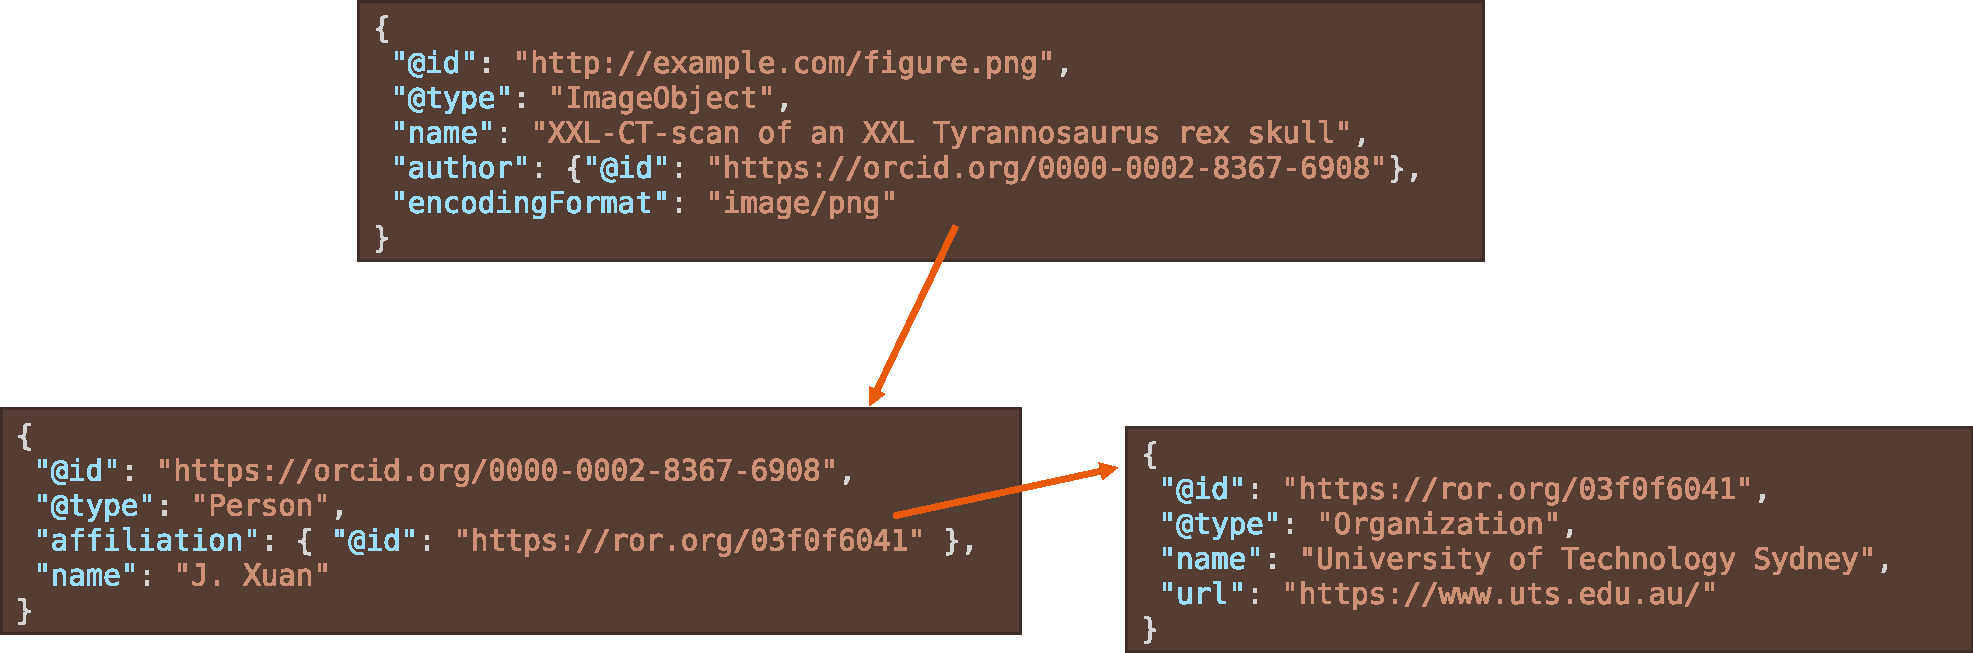
\includegraphics[width=\textwidth]{figures/ch03/jsonld.pdf}
    \caption[Example of linked RDF resources]{\textbf{Example of linked RDF resources}. Each \emph{resource} in an RDF graph has an identifier, here shown as absolute URIs, a type and a series of properties. A property value can either be a \emph{literal} (e.g. "Josiah Carberry") or another resource (e.g. \url{https://ror.org/03f0f6041}). A graph is formed by such cross-references across resources.
    In the idealised Semantic Web, every URI would resolve to a description of its resource in RDF. In practice there can be misalignments of identifiers, vocabularies, resolution mechanisms, or simply lack of RDF adoptation. Therefore any RDF graph can describe any Web resource identified by its URI, and these descriptions, using an \emph{open world assumption} \cite{Drummond 2006}, can be merged with other graphs describing the same resource.
    For brevity and comparison from later chapters this figure uses the newer RDF format JSON-LD \cite{w3-json-ld}, 
    which can be expanded with context \url{http://schema.org/} (not shown) to anchor types and 
    properties as absolute URIs and generate corresponding RDF triples (listing \vref{ch3:triples}). 
    }
  \label{ch3:fig:jsonld}
\end{figure}

\begin{listing}
  \footnotesize
  \begin{verbatim}
<http://example.com/figure.png> a <http://schema.org/ImageObject> .
<http://example.com/figure.png> <http://schema.org/name> "XXL-CT-scan of an XXL Tyrannosaurus rex skull" .
<http://example.com/figure.png> <http://schema.org/author> <https://orcid.org/0000-0002-1825-0097> .
<http://example.com/figure.png> <http://schema.org/encodingFormat> "image/png" .

<https://orcid.org/0000-0002-1825-0097> a <http://schema.org/Person> .
<https://orcid.org/0000-0002-1825-0097> <http://schema.org/name> "Josiah Carberry" .
<https://orcid.org/0000-0002-1825-0097> <http://schema.org/affiliation> <https://ror.org/03f0f6041> .

<https://ror.org/03f0f6041> a <http://schema.org/Organization> .
<https://ror.org/03f0f6041> <http://schema.org/name> "University of Technology Sydney" .
<https://ror.org/03f0f6041> <http://schema.org/url> "https://www.uts.edu.au/" .
  \end{verbatim}  
  \caption[Example of RDF triples]{\textbf{Example of RDF triples} corresponding to figure \vref{ch3:fig:jsonld} after expansion with a JSON-LD context. In this example the properties and types are all using the same vocabulary \cite{schema.org}, in the traditional Semantic Web it is common to mix vocabularies. This listing uses the RDF syntax N-Triples \cite{n-triples} where each line indicates \emph{subject}, \emph{predicate} and \emph{object}. Notable here is the syntactical difference between an URI reference that is part of the graph \texttt{<https://ror.org/03f0f6041>} and a string literal \texttt{"https://www.uts.edu.au/"} which just happens to be a URI. }
  \label{ch3:triples}
\end{listing}

The early days of the Semantic Web saw fairly lightweight approaches with the establishment of vocabularies such as FOAF (to describe people and their affiliations) and Dublin Core (for bigbliographic data). Vocabularies themselves were formalised using RDFS or simply as human-readable HTML web pages defining each term. The main approach of this \emph{Web of Data} was that a URI identified a \emph{resource} (e.g.~an author) with a HTML \emph{representation} for human readers, along with a RDF representation for machine-readable data of the same resource. By using \emph{content negotiation} in HTTP\footnote{\url{https://developer.mozilla.org/en-US/docs/Web/HTTP/Content_negotiation}}, the same identifier could be used in both views, avoiding \texttt{index.html} vs \texttt{index.rdf} exposure in the URLs. The concept of \emph{namespaces} gave a way to give a group of RDF resources with the same URI base from a Semantic Web-aware service a common \emph{prefix}, avoiding repeated long URLs.

The mid-2000s saw large academic interest and growth of the Semantic Web, with the development of more formal representation system for ontologies, such as OWL \cite{w3-owl2-overview}, allowing complex class hierarchies and logic inference rules following \emph{open world} paradigm. (e.g.~a \emph{ex:Parent} is equivalent to a subclass of \emph{foaf:Person} which must \emph{ex:hasChild} at least one \emph{foaf:Person}, then if we know \emph{:Alice a ex:Parent} we can infer \emph{:Alice ex:hasChild {[}a foaf:Person{]}} even if we don't know who that child is). More human-readable syntaxes for RDF such as Turtle evolved at this time, and conferences such as \footurl{https://iswc2022.semanticweb.org/}{ISWC} \cite{horrocksSemanticWebISWC2002} gained traction, with a large interest in knowledge representation and logic systems based on Semantic Web technologies evolving at the same time.

Established Semantic Web services and standards include: SPARQL \cite{w3-sparql11-overview} (pattern-based triple queries), \footurl{https://www.w3.org/TR/rdf11-concepts/\#section-dataset}{named graphs} \cite{w3-rdf11-concepts} (triples expanded to \emph{quads} to indicate statement source or represent conflicting views), triple/quad stores (graph databases such as OpenLink Virtuoso, GraphDB, 4Store), mature RDF libraries (including Redland RDF, Apache Jena, Eclipse RDF4J, RDFLib, RDF.rb, rdflib.js), and graph visualisation.

RDF is one way to implement \emph{knowledge graphs}, a system of named edges and nodes\footnote{In RDF, each triple represent an edge that is named using its property URI, and the nodes are subject/object as URIs, blank nodes or (for objects) typed literal values \cite{w3-rdf11-primer}.} \cite{nurdiati2008}, which when used to represent a sufficiently detailed model of the world, can then be queried and processed to answer detailed research questions. The creation of RDF-based knowledge graphs grew particularly in fields like bioinformatics, e.g.~for describing genomes and proteins \cite{gobleStateNationData2008c,williamsOpenPHACTSSemantic2012c}. In theory, the use of RDF by the life sciences would enable interoperability between the many data repositories and support combined views of the many aspects of bio-entities -- however in practice most institutions ended up making their own ontologies and identifiers, for what to the untrained eye would mean roughly the same. One can argue that the toll of adding the semantic logic system of rich ontologies meant that small, but fundamental, differences in opinion (e.g.~\emph{should a gene identifier signify just the particular DNA sequence letters, or those letters as they appear in a particular position on a human chromosome?}) led to large differences in representational granularity, and thus needed different identifiers.

Facing these challenges, thanks to the use of universal identifiers in the form of URIs, \emph{mappings} could retrospectively be developed not just between resources, but also across vocabularies. Such mappings can be expressed themselves using lightweight and flexible RDF vocabularies such as SKOS \cite{w3-skos-primer} (e.g.~\texttt{dct:title\ skos:closeMatch\ schema:name} to indicate near equivalence of two properties). Exemplifying the need for such cross-references, automated ontology mappings have identified large potential overlaps, like 372 definitions of \texttt{Person}) \cite{huHowMatchableAre2011a}.


The move towards \emph{Open Science} data sharing practices did from the late 2000s encourage knowledge providers to distribute collections of RDF descriptions as downloadable \emph{datasets} \footnote{\emph{Datasets} that distribute RDF graphs should not be confused with \emph{RDF Datasets} used for partitioning \emph{named graphs}, see \url{https://www.w3.org/TR/rdf11-concepts/\#section-dataset}}, so that their clients can avoid thousands of HTTP requests for individual resources\label{ch20:avoid-lots-of-requests}. This enabled local processing, mapping and data integration across datasets (e.g.~Open PHACTS \cite{grothAPIcentricLinkedData2014b}), rather than relying on the providers' RDF and SPARQL endpoints (which could become overloaded when handling many concurrent, complex queries).

With these trends, an emerging problem was that adopters of the Semantic Web primarily utillised it as a set of graph technologies, with little consideration to existing Web resources. This meant that links stayed mainly within a single information system, with little URI reuse even with large term overlaps \cite{kamdarSystematicAnalysisTerm2017a}. Just like \emph{link rot} affect regular Web pages and their citations from scholarly communication \cite{kleinScholarlyContextNot2014a}, for a majority of described RDF resources in the \footurl{https://lod-cloud.net/}{Linked Open Data} (LOD) Cloud's gathering of more than thousand datasets, unfortunately do not actually link to (still) downloadable (\emph{dereferenceable}) Linked Data \cite{polleresMoreDecentralizedVision2020a}. Another challenge facing potential adopters is the plethora of choices, not just to navigate, understand and select to reuse the many possible vocabularies and ontologies \cite{carrieroLandscapeOntologyReuse2020a}, but also technological choices on RDF serialisation (at least \footurl{https://www.w3.org/TR/rdf11-primer/\#section-graph-syntax}{7 formats}), type system (RDFS \cite{w3-rdf-schema}, OWL \cite{w3-owl2-overview}, OBO \cite{tirmiziMappingOBOOWL2011a}, SKOS \cite{w3-skos-primer}), and deployment challenges \cite{sauermannCoolURIsSemantic2011} (e.g. hash vs slash in namespaces, HTTP status codes and PID redirection strategies).

\subsection{Linked Data: Rebuilding the Web of Data}\label{ch3:ld-web}

The \textbf{Linked Data} (LD) concept \cite{Bizer 2009} was kickstarted as a set of best practices \cite{LinkedDataDesign} to bring the Web aspect of the Semantic Web back into focus. Crucial to Linked Data is the \emph{reuse of existing URIs}, rather than making new identifiers. This means a loosening of the semantic restrictions previously applied, and an emphasis on building navigable data resources, rather than elaborate graph representations.

Vocabularies like \footurl{https://schema.org/}{schema.org} evolved not long after, intended for lightweight semantic markup of existing Web pages, primarily to improve search engines' understanding of types and embedded data. In addition to several such embedded \emph{microformats} \cite{OpenGraphProtocol,w3-rdfa-primer,HTMLStandard}, we find JSON-LD \cite{w3-json-ld} as a Web-focused RDF serialisation that aims for improved programmatic generation and consumption, including from Web applications. JSON-LD is as of 2023-05-18 used\footnote{Presumably this large uptake of JSON-LD is mainly for the purpose of Search Engine Optimisation (SEO), with typically small amounts of metadata which may not constitute Linked Data as introduced above, however this deployment nevertheless constitute machine-actionable structured data.} by 45\% of the top 10 million websites \cite{UsageStatisticsJSONLD}.

Recently there has been a renewed emphasis to improve the \emph{Developer Experience} \cite{DesigningLinkedData2018} for consumption of Linked Data, for instance RDF Shapes -- expressed in SHACL \cite{w3-shacl} or ShEx \cite{ShapeExpressionsShEx} -- can be used to validate RDF Data \cite{gayoValidatingRDFData2017a,thorntonUsingShapeExpressions2019a} before consuming it programmatically, or reshaping data to fit other models. While a varied set of tools for Linked Data consumptions have been identified, most of them still require developers to gain significant knowledge of the underlying Semantic Web technologies, which hampers adaption by non-LD experts \cite{klimekSurveyToolsLinked2019a}, which then tend to prefer non-semantic two-dimensional formats such as CSV files.

A valid concern is that the Semantic Web research community has still not fully embraced the Web, and that the ``final 20\%'' engineering effort is frequently overlooked in favour of chasing new trends such as Big Data and AI, rather than making powerful Linked Data technologies available to the wider groups of Web developers \cite{verborghSemanticWebIdentity2020a}. One bridging gap here by the Linked Data movement has been ``Linked Data by stealth'' approaches such as structured data entry spreadsheets powered by ontologies \cite{wolstencroftRightFieldEmbeddingOntology2011b}, the use of Linked Data as part of REST Web APIs \cite{pageRESTLinkedData2011}, and as shown by the big uptake by publishers to annotate the Web using schema.org \cite{bernsteinNewLookSemantic2016a}, with vocabulary use patterns documented by copy-pastable JSON-LD examples, rather than by formalised ontologies or developer requirements to understand the full Semantic Web stack.

Linked Data provides technologies that have evolved over time to satisfy its primary purpose of data interoperability. The needs to embrace the Web and developer experience have been central lessons learned.  In contrast, FDO is a new approach with many different potential paths forward, and having a partial overlap with the aims of Linked Data
